\indent 実験3では, 認証機構の処理能力(計算効率)を評価するための実験を行った. 
はじめに, ECDSAとEdDSAが1回の署名の生成, 検証にかかる時間を計測し, 
その後, 不正ノードの存在しない環境でノード数を37, 74, 112, 148, 185に設定して
250回ずつシミュレーションを行い, それぞれの実行にかかった時間と使用したメモリ量を調べた. 
実験2の主なシミレーションパラメータは表\ref{tab:exp3-params}に示す通りである. 
\indent 実験の結果は以下の通りである. 
\begin{longtable}{cc}
  \caption{実験3のシミュレーションパラメータ}
  \label{tab:exp3-params}
  \endfirsthead
  \hline
  シミュレーション時間 & 300[s] \\
  ノード数 & 37,74, 112, 148, 185 \\
  送受信ノードのペア数 & 1 \\ 
  不正ノード & なし \\ \hline
\end{longtable}

\begin{longtable}{c|cc}
  \caption{1回の署名作成, 署名検証にかかった時間}
  \label{tab:exp3_sigtime} \\
  \endfirsthead
  \hline
  プロトコル & 署名作成時間 $[ms]$ & 署名検証時間 $[ms]$ \\ \hline
  ECDSA & $0.371$ & $0.336$ \\
  EdDSA & $0.031$ & $0.097$ \\ \hline
\end{longtable}


\begin{figure}
  \centering
  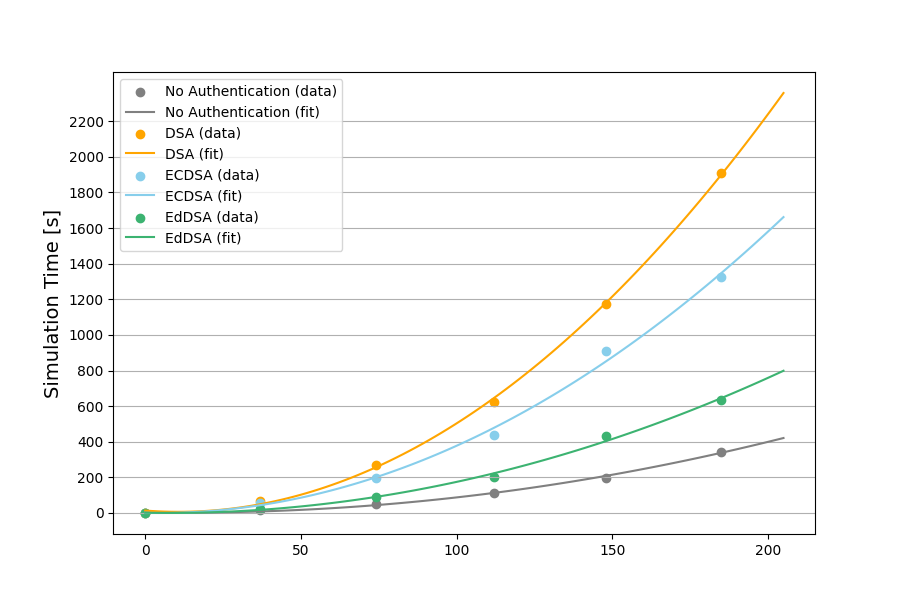
\includegraphics[width=1\textwidth]{figures/exp3_simtime.png}
  \caption{ノード数によるシミュレーション実行時間の変化}
  \label{fig:exp3_simtime}
\end{figure}
\clearpage
\setlength{\tabcolsep}{4pt}
\begin{longtable}{
    >{\raggedright\arraybackslash}p{3cm}
    >{\raggedright\arraybackslash}p{3.7cm}
    >{\raggedright\arraybackslash}p{2.5cm}
    >{\raggedright\arraybackslash}p{2.5cm}
    >{\raggedright\arraybackslash}p{2.5cm}
  }
  \caption{シミュレーション実行時間}
  \label{tab:exp3_simtime} \\
  \endfirsthead
  \hline
  % \multicolumn{1}{c}{Number of nodes} &
  % \multicolumn{1}{c}{No Authentication [s]} &
  % \multicolumn{1}{c}{DSA [s]} &
  % \multicolumn{1}{c}{ECDSA [s]} &
  % \multicolumn{1}{c}{Ed25519 [s]} \\ \hline \hline
  Number of nodes & No Authentication $[s]$ & ECDSA $[s]$ & EdDSA $[s]$ \\ \hline \hline
  \multicolumn{1}{c}{$37$} &
  \multicolumn{1}{c}{$14.1802$} &
  \multicolumn{1}{l}{$55.0108$} &
  \multicolumn{1}{l}{$24.4069$} \\
  \multicolumn{1}{c}{$74$} &
  \multicolumn{1}{c}{$50.5984$} &
  \multicolumn{1}{l}{$194.408$} &
  \multicolumn{1}{l}{$89.2728$} \\
  \multicolumn{1}{c}{$112$} &
  \multicolumn{1}{c}{$110.405$} &
  \multicolumn{1}{l}{$436.926$} &
  \multicolumn{1}{l}{$200.901$} \\
  \multicolumn{1}{c}{$148$} &
  \multicolumn{1}{c}{$196.971$} &
  \multicolumn{1}{l}{$910.373$} &
  \multicolumn{1}{l}{$431.346$} \\
  \multicolumn{1}{c}{$185$} &
  \multicolumn{1}{c}{$345.059$} &
  \multicolumn{1}{l}{$1324.55$} &
  \multicolumn{1}{l}{$635.155$} \\ \hline

  % $37$ & $14.1802$ & $69.9882$ & $55.0108$ & $24.4069$ \\
  % $74$ & $50.5984$ & $267.433$ & $194.408$ & $89.2728$ \\
  % $112$ & $110.405$ & $625.504$ & $436.926$ & $200.901$ \\
  % $148$ & $196.971$ & $1172.57$ & $910.373$ & $431.346$ \\
  % $185$ & $345.059$ & $1908.7$ & $1324.55$ & $635.155$ \\ \hline
\end{longtable}

\begin{figure}
  \centering
  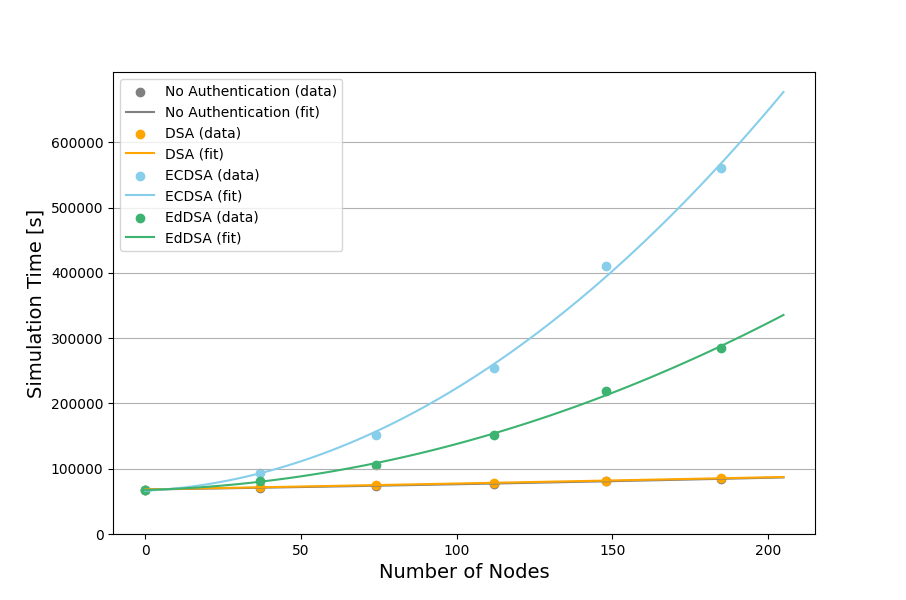
\includegraphics[width=1\textwidth]{figures/exp3_memory.png}
  \caption{ノード数によるメモリ使用量の変化}
  \label{fig:memory_usages}
\end{figure}

\clearpage
\setlength{\tabcolsep}{4pt}
\begin{longtable}{c|cccc}
  \caption{メモリ使用量}
  \label{tab:exp3_memory} \\
  \endfirsthead
  \hline
  Number of nodes & No Authentication [KB] & ECDSA [KB] & EdDSA [KB] \\ \hline \hline
  $37$ & 70,939 & 93,749 & 80,647 \\
  $74$ & 74,089 & 151,853 & 106,442 \\
  $112$ & 77,070 & 254,247 & 151,401 \\
  $148$ & 80,749 & 409,965 & 219,102 \\
  $185$ & 84,548 & 560,753 & 285,191 \\ \hline
\end{longtable}




\indent 表\ref{tab:exp3_sigtime}は, ECDSAとEdDSAにおいて, 
1回の署名作成と署名検証に要する時間を示したものである.
図\ref{fig:exp3_simtime}はシミュレーションパターンごとのノード数による
実行時間の変化を近似してグラフにしたものを, 表\ref{tab:exp3_simtime}はその具体的な
値を示したものである. 図\ref{fig:memory_usages}は, ノード数によるメモリ使用量の変化を近似して
グラフにしたものを, 表\ref{tab:exp3_memory}はその具体的な値を示したものである. \\
\indent 表\ref{tab:exp3_sigtime}より, EdDSAがECDSAに比べて署名生成, 署名検証にかかる時間が
短いことから, EdDSAはECDSAよりも高速に処理されることがわかった. 
図\ref{fig:exp3_simtime}, 表\ref{tab:exp3_sigtime}, 図\ref{fig:memory_usages}, 
表\ref{tab:exp3_memory}より, 同じノード数の場合において, EdDSAはECDSAよりも
シミュレーション実行時間やメモリ使用量が常に短い. さらに, シミュレーション実行時間と
メモリ使用量を示すグラフに描かれているEdDSAの近似曲線はECDSAの
近似曲線よりも勾配が緩やかである. これらの結果から, EdDSAはECDSAと比べて, 
ネットワーク全体の計算コストの増加を抑えつつ, より少ないリソースで効率的に動作することが可能であるため, 
特に大規模なネットワーク環境において優れたスケーラビリティを有すると考えられる. \\


